% Versão 0.9.15, 30/03/2020

% Este documento destina-se a servir como modelo para a produção de documentos
% de pesquisa do PPGINF/UFPR, como projetos, dissertações e teses. A classe de
% documento se chama "ppginf" (arquivo ppginf.cls) e define o formato básico do
% documento. O texto está organizado em capítulos que são colocados em
% subdiretórios separados. São definidos exemplos para a inclusão de figuras,
% códigos-fonte e a definição de tabelas.
%
% Produzido por Carlos Maziero (maziero@inf.ufpr.br).

%=====================================================

% Opções da classe ppginf:
%
% - defesa    : versão para entregar à banca; tem espaçamento 1,5
%               e omite algumas páginas iniciais (agradecimentos, etc)
% - final     : versão pós-defesa, para enviar à biblioteca;
%               tem espaçamento simples e todas as páginas iniciais.
% - oneside   : somente frente; use quando for gerar somente o PDF.
% - twoside   : frente/verso; use se precisar de uma versão impressa.
% - metadados : inclui metadados no PDF (por default não inclui)
% - ...       : demais opções aceitas pela classe "book"

% ATENÇÂO: este modelo tem suporte para português e inglês.
% As duas línguas devem ser informadas como opção da classe;
% a língua principal do documento deve vir POR ÚLTIMO.

% Versão de defesa
\documentclass[defesa,oneside,english,brazilian]{ppginf}

% Versão de defesa em inglês
%\documentclass[defesa,oneside,brazilian,english]{ppginf}

% Versão final em PDF para a biblioteca da UFPR
%\documentclass[final,oneside,english,brazilian]{ppginf}

% Versão final para impressão (frente/verso)
%\documentclass[final,twoside,english,brazilian]{ppginf}

% configurações de diversos pacotes, inclusive o fonte principal do texto
% Pacotes usados neste documento e suas respectivas configurações

% ------------------------------------------------------------------------------

% Definição de fontes

% formato dos arquivos-fonte (utf8 no Linux e latin1 no Windows)
\usepackage[utf8]{inputenc}	% arquivos LaTeX em Unicode (UTF8)

% usar codificação T1 para ter caracteres acentuados corretos no PDF
\usepackage[T1]{fontenc}

% fonte usada no corpo do texto (descomente apenas uma)
\usepackage{newtxtext,newtxmath}	% Times (se não tiver, use mathptmx)
%\usepackage{lmodern}			% Computer Modern (fonte clássico LaTeX)
%\usepackage{kpfonts}			% Kepler/Palatino (idem, use mathpazo)
%\renewcommand{\familydefault}{\sfdefault} % Arial/Helvética (leia abaixo)

% A biblioteca central da UFPR recomenda usar Arial, seguindo a recomendação da
% ABNT. Essa é uma escolha ruim, pois fontes sans-serif são geralmente inade-
% quados para textos longos e impressos, sendo melhores para páginas Web.
% http://www.webdesignerdepot.com/2013/03/serif-vs-sans-the-final-battle/.

% fontes usadas em ambientes específicos
\usepackage[scaled=0.9]{helvet}		% Sans Serif
\usepackage{courier}			% Verbatim, Listings, etc

% ------------------------------------------------------------------------------

% inclusão de figuras em PDF, PNG, PS, EPS
\usepackage{graphicx}

% subfiguras (subfigure is deprecated, don't use it)
\usepackage[labelformat=simple]{subcaption}
\renewcommand\thesubfigure{(\alph{subfigure})}

% ------------------------------------------------------------------------------

% inclusão/formatação de código-fonte (programas)
\usepackage{listings}
\lstset{language=c}
\lstset{basicstyle=\ttfamily\footnotesize,commentstyle=\textit,stringstyle=\ttfamily}
\lstset{showspaces=false,showtabs=false,showstringspaces=false}
\lstset{numbers=left,stepnumber=1,numberstyle=\tiny}
\lstset{columns=flexible,mathescape=true}
\lstset{frame=single}
\lstset{inputencoding=utf8,extendedchars=true}
\lstset{literate={á}{{\'a}}1  {ã}{{\~a}}1 {à}{{\`a}}1 {â}{{\^a}}1
                 {Á}{{\'A}}1  {Ã}{{\~A}}1 {À}{{\`A}}1 {Â}{{\^A}}1
                 {é}{{\'e}}1  {ê}{{\^e}}1 {É}{{\'E}}1  {Ê}{{\^E}}1
                 {í}{{\'\i}}1 {Í}{{\'I}}1
                 {ó}{{\'o}}1  {õ}{{\~o}}1 {ô}{{\^o}}1
                 {Ó}{{\'O}}1  {Õ}{{\~O}}1 {Ô}{{\^O}}1
                 {ú}{{\'u}}1  {Ú}{{\'U}}1
                 {ç}{{\c{c}}}1 {Ç}{{\c{C}}}1 }

% ------------------------------------------------------------------------------

% formatação de algoritmos
\usepackage{algorithm,algorithmic}
\iflanguage{brazilian} {\floatname{algorithm}{Algoritmo}}{}
\renewcommand{\algorithmiccomment}[1]{~~~// #1}
%\algsetup{linenosize=\footnotesize,linenodelimiter=.}

% ------------------------------------------------------------------------------

% listas de símbolos e de abreviações (a fazer)
%\usepackage[titles]{tocloft}
%\newlistof[part]{symb}{los}{Lista de Símbolos}
%\newlistof[part]{abbrev}{loa}{Lista de Abreviações}
%\newcommand{\symb}[2]{%
%\refstepcounter{symb}
%\addcontentsline{los}{symb}{\protect #1 :#2}\par}

% ------------------------------------------------------------------------------

% formatação de bibliografia
\usepackage{natbib}		% bibliografia no estilo NatBib

% ------------------------------------------------------------------------------

% outros pacotes diversos
\usepackage{alltt,moreverb}	% mais comandos no modo verbatim
\usepackage{lipsum}		% gera texto aleatório (para os exemplos)
\usepackage{currfile}		% infos sobre o arquivo/diretório atual
\usepackage[final]{pdfpages}	% inclusão de páginas em PDF
\usepackage{longtable}		% tabelas multi-páginas (tab símbolos/acrônimos)

% ------------------------------------------------------------------------------



%=====================================================

\begin {document}

% Principais dados, usados para gerar as páginas iniciais.
% Campos não utilizados podem ser removidos ou comentados.

% título
\title{Um modelo \LaTeX\ para dissertações e teses \\ (escrevi um título mais longo para ver como se comporta a quebra de linhas e o espaçamento entre elas)}

% palavras-chave e keywords (p/ resumo, abstract e metadados do PDF)
\pchave{Palavra-chave 1. Palavra-chave 2. Palavra-chave 3.}
\keyword{Keyword 1. Keyword 2. Keyword 3.}

% autoria
\author{Carlos Alberto Maziero}
\advisor{Donald Knuth}
\coadvisor{Leslie Lamport}

% instituição
\IfLanguageName{brazilian}
  { \instit{UFPR}{Universidade Federal do Paraná} }
  { \instit{UFPR}{Federal University of Paraná} }

% área de concentração (default do PPGInf, não mudar)
\IfLanguageName{brazilian}
  { \field{Ciência da Computação} }
  { \field{Computer Science} }

% data (só o ano)
\date{2018}

% local
\IfLanguageName{brazilian}
  { \local{Curitiba PR} }
  { \local{Curitiba PR - Brazil} }

% imagem de fundo da capa (se não desejar, basta comentar)
\coverimage{0-iniciais/fundo-capa.jpg}

%=====================================================

%% Descrição do documento (obviamente, descomentar somente UMA!)

% Por exigência da biblioteca da UFPR, a descrição do documento deve ser
% em português, mesmo em documentos em outras línguas. Vá entender...

% tese de doutorado
\descr{Tese apresentada como requisito parcial à obtenção do grau de Doutor em Ciência da Computação no Programa de Pós-Graduação em Informática, Setor de Ciências Exatas, da Universidade Federal do Paraná}

% exame de qualificação de doutorado
%\descr{Documento apresentado como requisito parcial ao exame de qualificação de Doutorado no Programa de Pós-Graduação em Informática, Setor de Ciências Exatas, da Universidade Federal do Paraná}

% dissertação de mestrado
%\descr{Dissertação apresentada como requisito parcial à obtenção do grau de Mestre em Informática no Programa de Pós-Graduação em Informática, Setor de Ciências Exatas, da Universidade Federal do Paraná}

% exame de qualificação de mestrado
%\descr{Documento apresentado como requisito parcial ao exame de qualificação de Mestrado no Programa de Pós-Graduação em Informática, Setor de Ciências Exatas, da Universidade Federal do Paraná}

% trabalho de conclusão de curso
%\descr{Trabalho apresentado como requisito parcial à conclusão do Curso de Bacharelado em XYZ, Setor de Ciências Exatas, da Universidade Federal do Paraná}

% trabalho de disciplina
%\descr{Trabalho apresentado como requisito parcial à conclusão da disciplina XYZ no Curso de Bacharelado em XYZ, Setor de Ciências Exatas, da Universidade Federal do Paraná}

% doctorate thesis
%\descr{Thesis presented as a partial requirement for the degree of Doctor in Computer Science in the Graduate Program in Informatics, Exact Sciences Sector, of the Federal University of Paraná, Brazil}

% doctorate qualification
%\descr{Document presented as a partial requirement for the doctoral qualification exam in the Graduate Program in Informatics, Exact Sciences Sector, of the Federal University of Paraná, Brazil}

% MSc dissertation
%\descr{Dissertation presented as a partial requirement for the degree of Master of Sciences in Informatics in the Graduate Program in Informatics, Exact Sciences Sector, of the Federal University of Paraná, Brazil.}

% MSc qualification
%\descr{Document presented as a partial requirement for the Master of Sciences qualification exam in the Graduate Program in Informatics, Exact Sciences Sector, of the Federal University of Paraná, Brazil}

%=====================================================

% define estilo das páginas iniciais (capas, resumo, sumário, etc)
\frontmatter
\pagestyle{frontmatter}

% produz capa e folha de rosto
\titlepage

% páginas que só aparecem na versão final (a inclusão é automática)
% IMPORTANTE: o conteúdo exato da ficha catalográfica é preparada pela
% Biblioteca da UFPR. Não "invente" um conteúdo para ela!

\begin{ficha}	% só gera conteúdo se for na versão final

% inclusão da ficha catalográfica final (arquivo PDF)
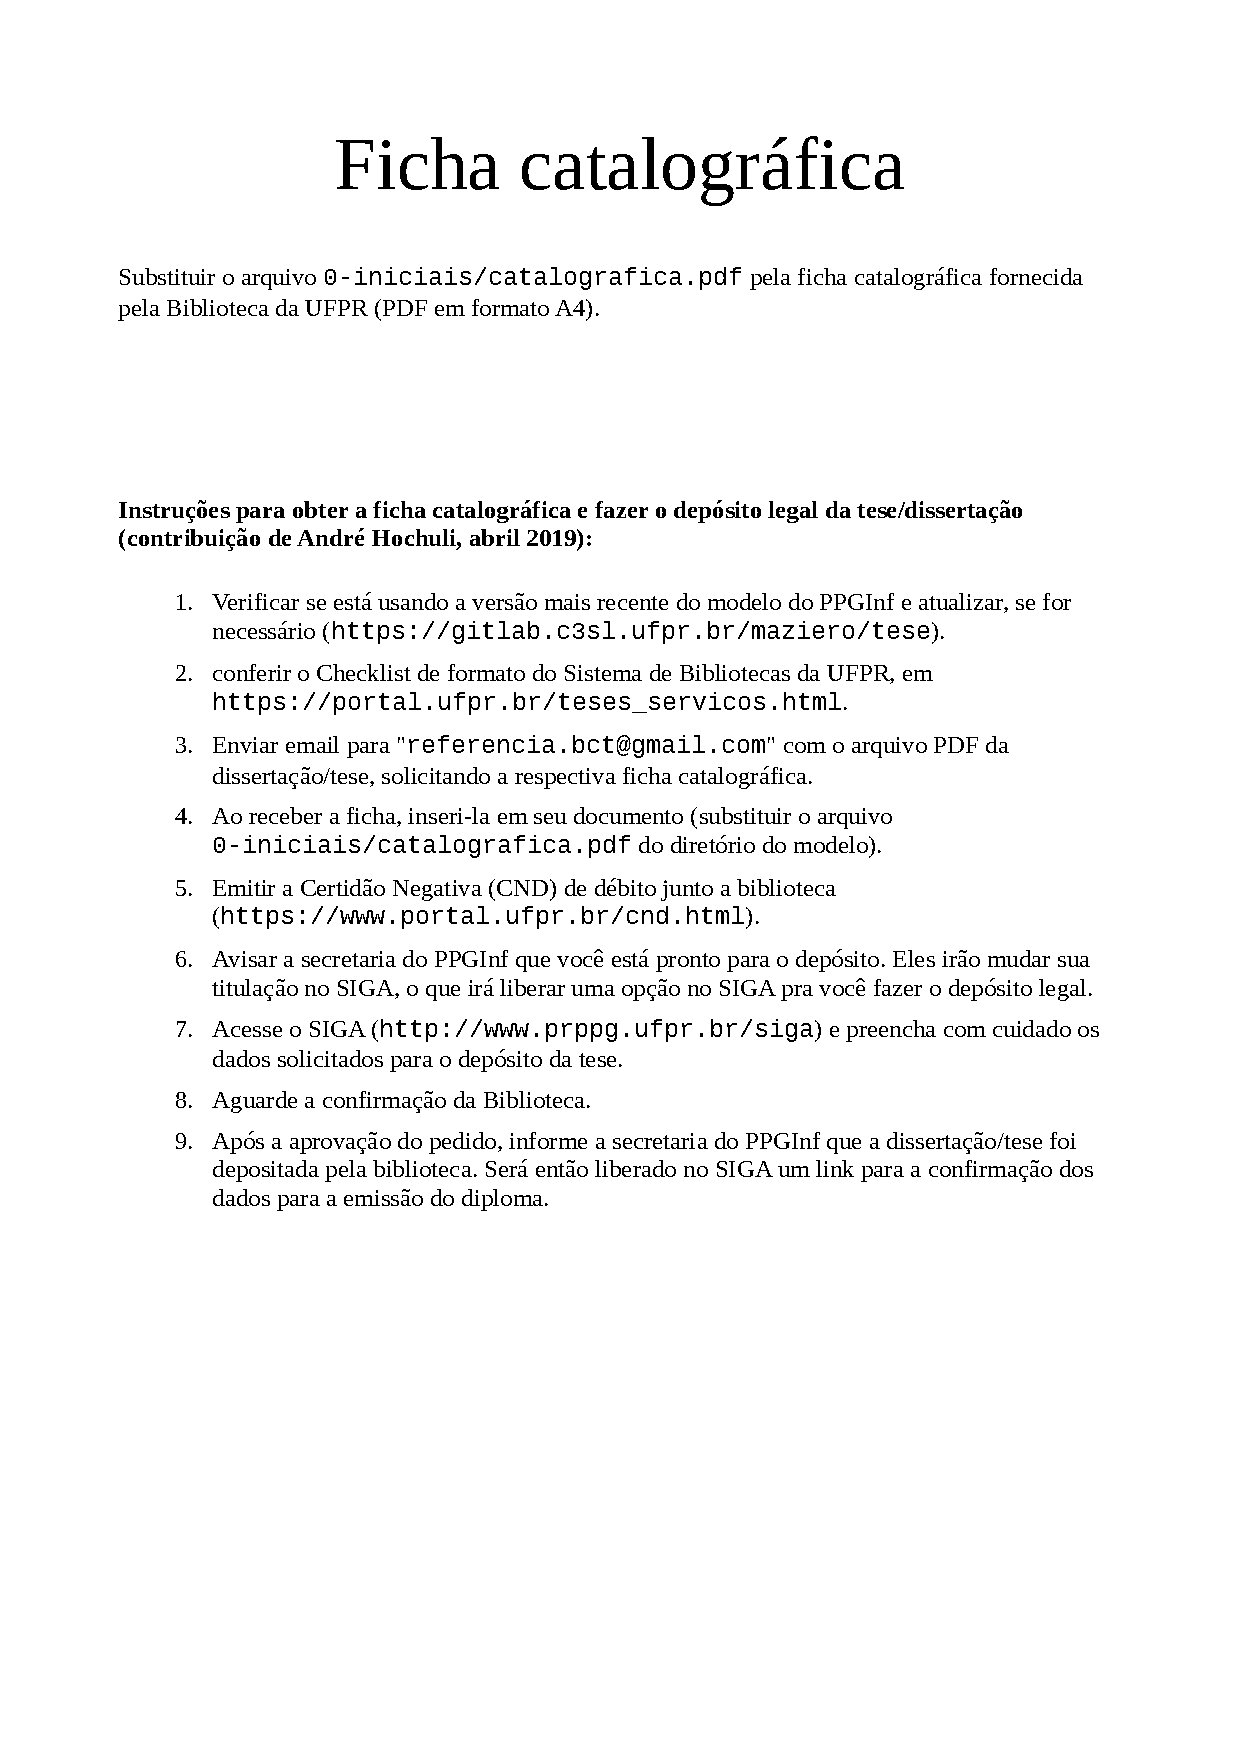
\includepdf[noautoscale]{0-iniciais/catalografica.pdf}

\end{ficha}

%=====================================================
	% ficha catalográfica
% A ficha de aprovação será fornecida pela secretaria do programa,
% após a defesa e cumprimento dos demais trâmites legais.

\begin{aprovacao}	% só gera conteúdo se for na versão final

% inclusão do termo de aprovação final (arquivo PDF)
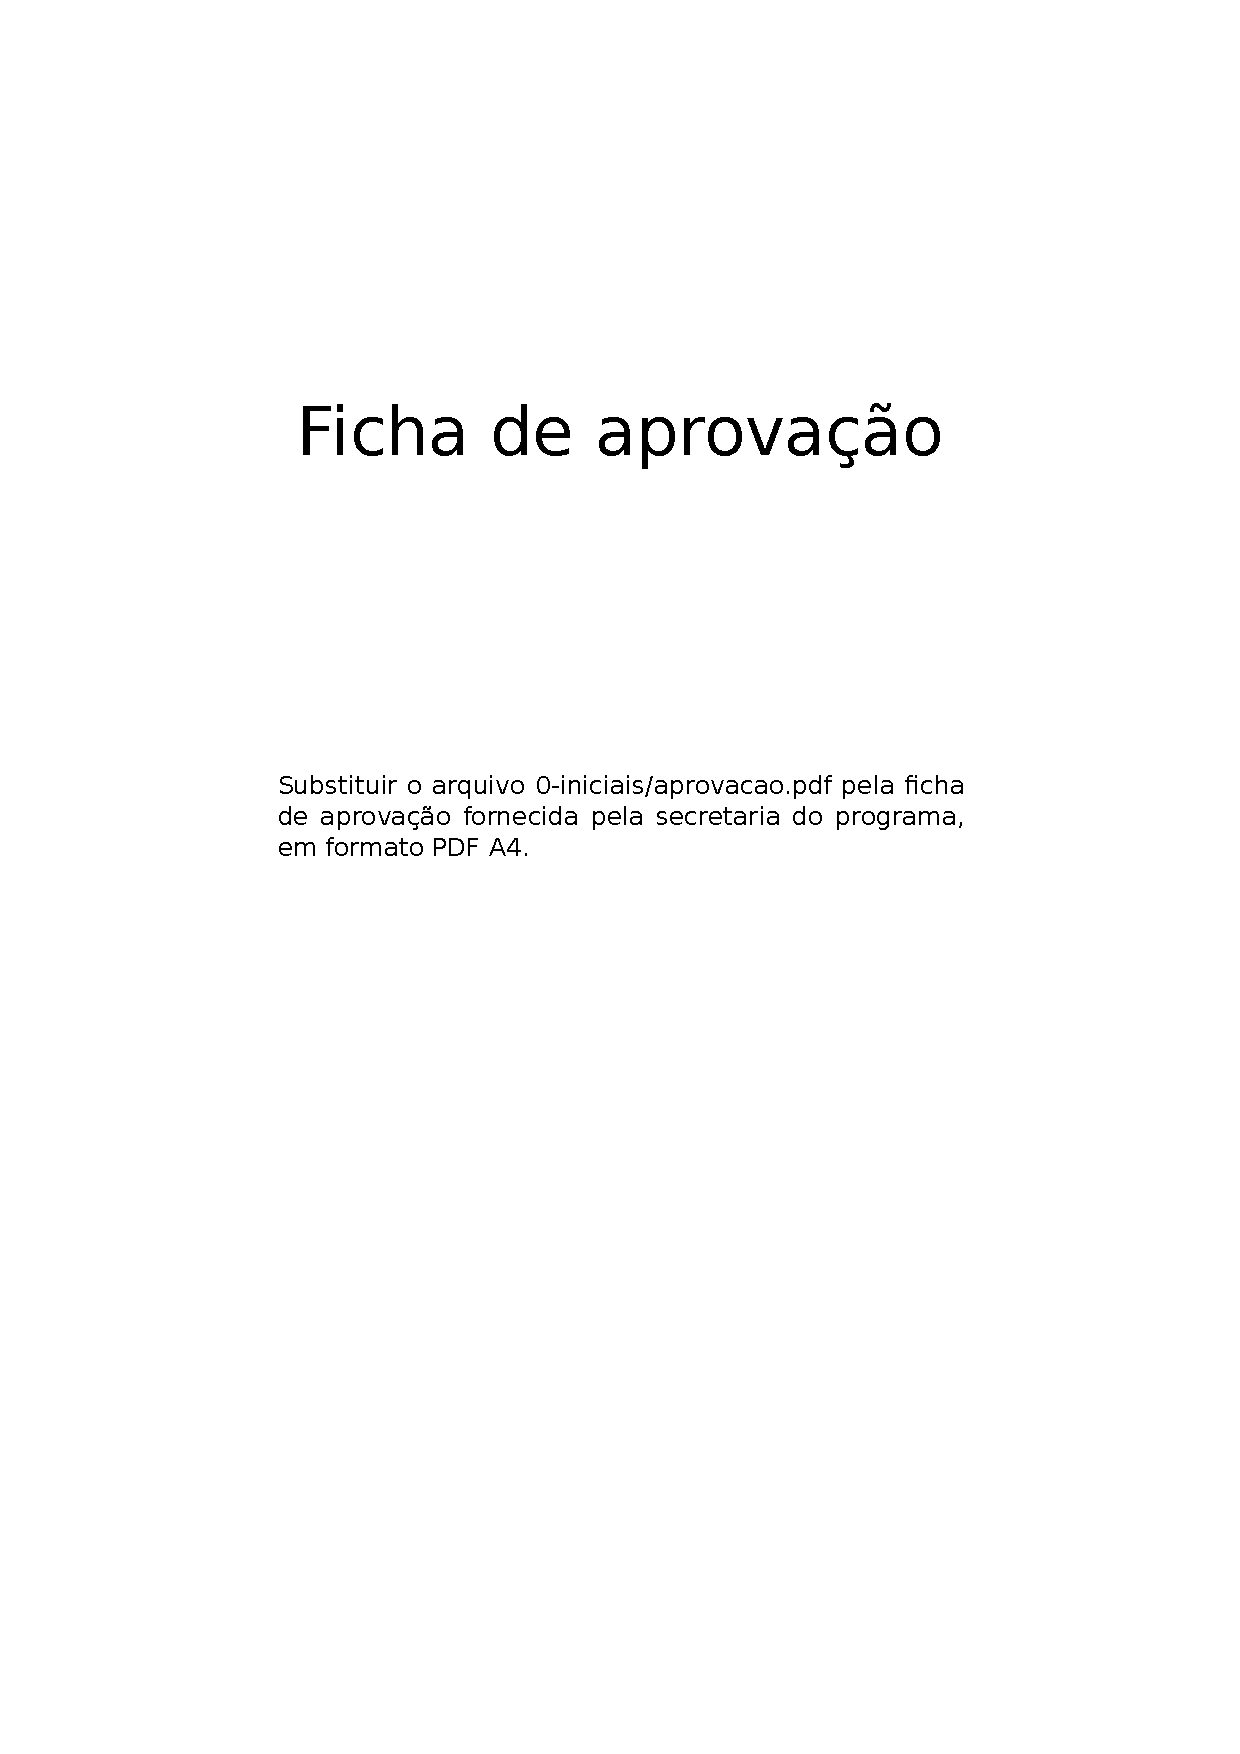
\includepdf[noautoscale]{0-iniciais/aprovacao.pdf}

\end{aprovacao}

%=====================================================
		% folha de aprovação
\begin{dedica}  % só gera conteúdo se for na versão final

A alguém...

\end{dedica}

		% dedicatória
\begin{agradece}	% só gera conteúdo se for na versão final

Inserir os agradecimentos. Os agradecimentos devem ocupar no máximo uma página, devem ser justificados na largura da página e com um afastamento de parágrafo na primeira linha de 1,27 cm. O espaçamento entre linhas deve ser de 1,5 linhas. Não deve haver espaçamento adicional entre parágrafos.

\lipsum[2-5]	% gera um texto aleatório

\end{agradece}

		% agradecimentos

% resumo (português) e abstract (inglês)
\begin{resumo}

Uma crescente preocupação com fatores climáticos e com o aquecimento global visando uma diminuição do consumo de combustíveis fósseis, vem abrindo espaço para o desenvolvimento de novos modelos na geração e consumo de energia. Uma evolução das fontes renováveis de energia trouxe a possibilidade de uma geração descentralizada, surgindo assim, o conceito da microrrede. Essas, trazem novas necessidades na manutenção da qualidade e no controle da energia elétrica em redes com geração intermitente, levando assim, ao uso de sistemas de armazenamento de energia. Além disso, o avanço na mobilidade elétrica, proporcionando uma maior densidade de energia das baterias, possibilitou o surgimento de veículos elétricos baratos e competitivos.

Desta forma, o objetivo deste trabalho foi o desenvolvimento de dois sistemas de armazenamento de energia, um conectado à microrrede do Departamento de Engenharia Elétrica (DELT) localizado no Centro Politécnico da Universidade Federal do Paraná (UFPR) em Curitiba e outra utilizada em um veículo elétrico do tipo Formula SAE, para competição nacional pela equipe UFPR Formula.

Primeiramente foi feito um estudo dos sistemas nos quais o armazenamento seria integrado, com uma revisão teórica do funcionamento dos principais componentes; foi então feito um estudo dos diferentes tipos e tecnologias de sistemas de armazenamento de energia, suas aplicações, características, estado da arte e aspectos de segurança; uma metodologia de organização do projeto foi definida: inicialmente definidos requerimentos para cada subsistema, depois projeto da arquitetura e integração do sistema, chegando na especificação do componente; e finalmente, como resultado se teve um projeto completo e especificado para os dois sistemas.

\end{resumo}

\begin{otherlanguage}{english}

\begin{abstract}

% em inglês, o primeiro parágrafo não deve ser indentado
\noindent
The abstract should be the English translation of the ``resumo'', no more, no less.

\end{abstract}

\end{otherlanguage}



% listas  de figuras, tabelas, abreviações/siglas, símbolos
\listoffigures				% figuras
\clearpage
\listoftables				% tabelas
%=====================================================

% lista de acrônimos (siglas e abreviações)

\begin{listaacron}

\begin{longtable}{p{0.2\linewidth}p{0.7\linewidth}}
DINF & Departamento de Informática\\
PPGINF & Programa de Pós-Graduação em Informática\\
UFPR & Universidade Federal do Paraná\\
\end{longtable}

\end{listaacron}

%=====================================================
		% acrônimos, deve ser preenchida à mão
%=====================================================

% lista de símbolos

\begin{listasimb}

\begin{longtable}{p{0.2\linewidth}p{0.7\linewidth}}
$\alpha$ & alfa, primeira letra do alfabeto grego\\
$\beta$ & beta, segunda letra do alfabeto grego\\
$\gamma$ & gama, terceira letra do alfabeto grego\\
$\omega$ & ômega, última letra do alfabeto grego\\
$\pi$ & pi \\
$\tau$ & Tempo de resposta do sistema\\
$\theta$ & Ângulo de incidência do raio luminoso\\
\end{longtable}

\end{listasimb}

%=====================================================
		% símbolos, idem
\tableofcontents			% sumário

%=====================================================

% define estilo do corpo do documento (capítulos e apêndices)
\mainmatter
\pagestyle{mainmatter}

% inclusao de cada capítulo, alterar a gosto (do professor de Metodologia)
\chapter{Introdução}

%=====================================================

% A introdução geral do documento pode ser apresentada através das seguintes seções: Desafio, Motivação, Proposta, Contribuição e Organização do documento (especificando o que será tratado em cada um dos capítulos). O Capítulo 1 não contém subseções\footnote{Ver o Capítulo \ref{cap-exemplos} para comentários e exemplos de subseções.}.

Este modelo foi proposto com o intuito de padronizar e simplificar as monografias, dissertações e teses produzidas no Departamento de Informática da UFPR. Ele foi vagamente inspirado nas normas da ABNT (conforme indicado em \cite{bibufpr15}), mas não as segue \emph{ipsis litteris}. Várias alterações foram feitas com o objetivo de melhorar sua estética e tornar o texto mais legível para trabalhos na área de informática. A versão atualizada deste modelo está disponível em \cite{maziero15}.

Este modelo está baseado em uma classe especifica \verb#ppginf.cls#, que aceita várias opções de compilação. A versão do documento pode ser:

\begin{itemize}

\item \verb#defesa#: é gerado um documento em espaço 1,5, frente simples e sem as páginas iniciais adicionais; é uma versão adequada para receber as anotações dos membros da banca de defesa.

\item \verb#final#: é gerado um documento em espaço simples, frente/verso, com páginas iniciais (capa, ficha catalográfica, folha de aprovação, agradecimentos, etc). É uma versão bem mais compacta, mais ecológica e ideal para a impressão definitiva.

\end{itemize}

Para obter os melhores resultados, compile este modelo usando a seguinte sequência de passos:

\begin{quote}
\begin{footnotesize}
\begin{verbatim}
pdflatex  main          // compilação inicial
bibtex main             // processa referências bibliográficas
pdflatex  main          // compilação final
\end{verbatim}
\end{footnotesize}
\end{quote}

ou

\begin{quote}
\begin{footnotesize}
\begin{verbatim}
make                    // faz tudo...
\end{verbatim}
\end{footnotesize}
\end{quote}

Os principais itens considerados na formatação deste documento foram:

\begin{itemize}

\item Papel em formato A4, com margens de 20 mm à direita e embaixo, 30 mm nos demais lados. Não devem ser usados cabeçalhos ou rodapés além dos que estão aqui propostos.

\item O texto principal do documento escrito em 12 pontos. O fonte principal do texto pode ser selecionado no arquivo \verb#packages.tex#.

\item Código-fonte, listagens e textos similares são formatados em fonte Courier 12 ou 10 pontos.

\item O espaçamento padrão entre linhas é 1,5 linhas (1 linha na versão final). Não inserir espaços adicionais entre parágrafos normais. Figuras, tabelas, listagens e listas de itens devem ter um espaço adicional antes e após os mesmos.

\item As páginas iniciais não são numeradas.

\item O corpo do texto é numerado com algarismos arábicos (1, 2, 3, ...) a partir da introdução, ate o final do documento. Os números de página devem estar situados no alto à direita (páginas direitas) ou à esquerda (páginas esquerdas).

\item Expressões em inglês, grego, latim ou outras línguas devem ser enfatizadas em itálico, como \emph{sui generis} ou \emph{scheduling} (use o comando \verb#\emph{...}#).

\item Para reforçar algo, deve-se usar somente \textbf{negrito}. \underline{Sublinhado} ou MAIÚSCULAS não devem ser usados como forma de ênfase!

\item As notas de rodapé também têm um modelo\footnote{As notas de rodapé dever ser escritas em tamanho 10 pt, numeradas em arábico.}. Notas de rodapé servem para fazer algum comentário paralelo; não as use para colocar URLs, referências bibliográficas ou significado de siglas.

\end{itemize}

Felizmente o \LaTeX\ resolve a maior parte dessas questões!

%=====================================================
			% introdução
\chapter{Alguns exemplos}
\label{cap:exemplos}

% figuras estão no subdiretório "figuras/" dentro deste capítulo
\graphicspath{\currfiledir/figuras/}

%=====================================================

\section{Guias de \LaTeX}

Este modelo contém exemplos para os padrões de inserção de figuras, tabelas, listas de itens, bibliografia, etc. Em caso de dúvidas ou discordância, Pode-se entrar em contato com a direção ou secretaria do programa. Obviamente, críticas (construtivas) e sugestões são muito bem-vindas.

Para aprender a usar \LaTeX, um bom guia introdutório disponível na Internet é \cite{oetiker07}, que também tem uma versão em português. Para tópicos mais avançados consulte \cite{goossens93}.

%=====================================================

\section{Estrutura do texto}

Para melhorar a legibilidade do texto, deve ser extremamente evitado o uso de subdivisões mais profundas que a subseção (por exemplo, subsubseções). Se elas forem absolutamente necessarias, não devem ser numeradas. Deve-se analisar a possibilidade de uso de uma lista de itens em seu lugar. O número de níveis de texto do documento não deve exceder três: capítulo, seção e subseção. O uso de mais que três níveis dificulta a leitura e prejudica muito a estética do texto.

%=====================================================

\section{Estilo de redação}

Ao elaborar o texto da dissertação ou da tese, o mais indicado é o uso do verbo na forma impessoal. Exemplos:

\begin{itemize}
\item ... utilizaram-se os seguintes dados ...
\item ... elaborou-se de forma precisa ...
\item ... trata-se os algoritmos ...
\item ... foram obtidos resultados significativos ...
\end{itemize}

Além disso, deve-se a todo custo evitar a ``linguagem de revista'', com expressões como ``sensacional'', ``impressionante'', ``monstruoso'', etc (por exemplo: ``Os resultados obtidos são sensacionais, sobretudo considerando a monstruosa margem de erro.'').

%=====================================================

\section{Exemplo de figura}

A forma sugerida para incluir figuras em um documento \LaTeX\ é importá-las usando o pacote \texttt{graphicx}. Como formatos gráficos sugere-se:

\begin{itemize}

\item Formatos \emph{raster}, como PNG (\emph{Portable Network Graphics}) ou JPG (\emph{Joint Photographic Experts Group}) para fotografias; procure usar uma resolução de ao menos 150 dpi (\emph{dots per inch}).

\item Formatos vetoriais, como PDF (\emph{Portable Document Format}) ou EPS (\emph{Extended PostScript}) para diagramas e gráficos\footnote{NUNCA use JPG ou GIF para desenhos vetoriais, pois o resultado final geralmente fica borrado.}.

\end{itemize}

A maior parte das ferramentas permite exportar figuras nesses formatos (a figura do exemplo foi produzida com o \emph{Inkscape}, um programa livre multiplataforma). A figura \ref{fig:comun-intra-inter} mostra um exemplo de inclusão de figura em PDF.

% exemplo de inserção de figura
\begin{figure}[!htb]
\centering
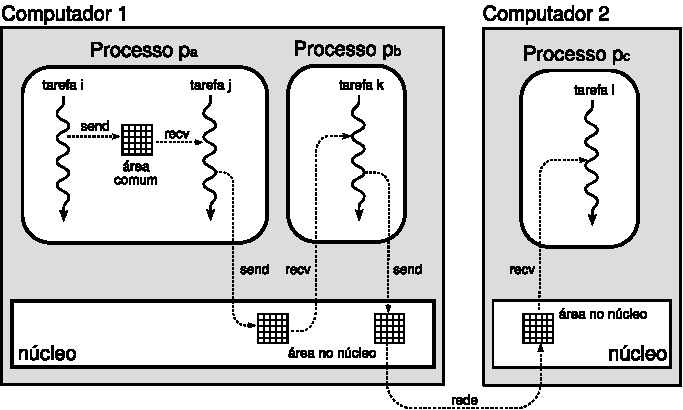
\includegraphics[width=12cm]{exemplo-figura.pdf}
\caption{Comunicação inter-processos.}
\label{fig:comun-intra-inter}
\end{figure}

Para mais informações consulte \cite{goossens93}.

%=====================================================

\section{Exemplo de tabela}

Tabelas são elementos importantes de um documento. No \LaTeX\ as tabelas podem ser objetos flutuantes (definidas no ambiente \texttt{table} e referenciadas por números usando \texttt{label} e \texttt{ref}) ou objetos fixos simples, criados pelo ambiente \texttt{tabular}. A tabela \ref{tab:modelos} é um exemplo de tabela flutuante, cuja posição no texto pode variar em função das quebras de página.

\begin{table}[!htp]
\centering
\caption{Os 16 modelos centrais do UCON$_{\mathrm{ABC}}$}
\label{tab:modelos}
\begin{tabular}{|c|cccc|}
\cline{2-5}
\multicolumn{1}{c|}{}& 0 (imutável) & 1 (\emph{pre-update}) & 2 (\emph{on-update}) & 3 (\emph{pos-update}) \\
\hline
\texttt{preA} & \textbullet & \textbullet & -- & \textbullet \\
\hline
\texttt{onA} & \textbullet & \textbullet & \textbullet & \textbullet \\
\hline
\texttt{preB} & \textbullet & \textbullet & -- & \textbullet \\
\hline
\texttt{onB} & \textbullet & \textbullet & \textbullet & \textbullet \\
\hline
\texttt{preC} & \textbullet & -- & -- & -- \\
\hline
\texttt{onC} & \textbullet & -- & -- & -- \\
\hline
\end{tabular}
\end{table}

%=====================================================

\section{Exemplo de equação}

Equações destacadas devem ser numeradas como mostra a equação \ref{eq:relatividade}:

\begin{equation}
E = m \times c^2
\label{eq:relatividade}
\end{equation}

%=====================================================

\section{Exemplos de código-fonte}

Códigos-fonte podem ser produzidos de forma simples através do ambiente \texttt{verbatim}, como mostra este exemplo:

\begin{footnotesize}
\begin{verbatim}
#include <stdio.h>

int main (int argc, char *argv[])
{
   int i ;                           // uma variavel local

   for (i=0; i< 100; i++)            // um laço for
      printf ("i vale %d\n", i) ;    // uma saída na tela
}
\end{verbatim}
\end{footnotesize}

No entanto, é preferível usar pacotes especializados para a edição ou inclusão de códigos-fonte, como o pacote \texttt{listings}. Eis um exemplo de código-fonte escrito com esse pacote:

% exemplo de código-fonte definido no próprio texto

\begin{lstlisting}
#include <stdio.h>

int main (int argc, char *argv[])
{
   int i ;                           // uma variável local

   for (i=0; i< 100; i++)            // um laço for
      printf ("i vale %d\n", i) ;    // uma saída na tela
}
\end{lstlisting}

Esse pacote também permite incluir códigos-fonte de arquivos externos. Eis um exemplo:

% exemplo de código-fonte incluso

\lstinputlisting{2-fundam/exemplo.c}

%=====================================================

\section{Exemplo de algoritmo}

Os pacotes \texttt{algorithm} e \texttt{algorithmic} permitem formatar algoritmos facilmente. Eis um exemplo:

\begin{algorithm}[H]
\caption{Ações de $s_i$ ao encerrar um ciclo:}
\label{alg:on-period-ending}
\begin{small}
\begin{algorithmic}[1]
\FORALL{$x \in \mathcal{K}_i$}
  \STATE{$\mathit{banned}_i(x) \gets$ FALSE}
  \STATE{$mi_i(x) \gets 0$}
  \STATE{$mm_i(x) \gets 0$}
  \STATE{$\mathit{age}_i(x) \gets \mathit{age}_i(x) + 1$}
  \IF{$\mathit{age}_i(x) = \mathit{age}_\mathit{max}$}
     \STATE{$\mathcal{K}_i \gets \mathcal{K}_i - \{x\}$}
     \COMMENT{``esquece'' do servidor $x$}
     \STATE{remove as informações locais sobre $x$}
     \STATE{envia $\mathit{notify}(x,\mathit{undef})$ ao grupo de confiança $\mathcal{T}_i$}
  \ENDIF
\ENDFOR
\end{algorithmic}
\end{small}
\end{algorithm}
 
%=====================================================

\section{Exemplo de citação}

Como afirmou Maquiavel em seu livro \emph{O Príncipe}:

\begin{quote}
``Nada é mais difícil de instituir, mais perigoso de conduzir, mais incerto no seu sucesso, do que liderar a introdução de uma nova ordem de coisas... O inovador faz inimigos em todos aqueles que prosperavam sobre as antigas regras, e somente tíbio suporte é esperado daqueles que prosperariam na novidade, porque os homens são geralmente incrédulos, nunca realmente confiam nas coisas novas, a menos que as tenham testado em experiência''.
\end{quote}

%=====================================================

\section{Conclusão}

Todo capítulo (com exceção da introdução e da conclusão) deve encerrar com uma pequena conclusão local, resumindo os tópicos apresentados no capítulo e preparando o leitor para o próximo capítulo (exceto se esse for a conclusão geral). Caso o capítulo tenha apresentado resultados obtidos pelo próprio autor, estes devem ser sucintamente relembrados aqui.

%=====================================================
		% fundamentação teórica
%\chapter{Alguns exemplos}
\label{cap:exemplos}

% figuras estão no subdiretório "figuras/" dentro deste capítulo
\graphicspath{\currfiledir/figuras/}

%=====================================================

\section{Guias de \LaTeX}

Este modelo contém exemplos para os padrões de inserção de figuras, tabelas, listas de itens, bibliografia, etc. Em caso de dúvidas ou discordância, Pode-se entrar em contato com a direção ou secretaria do programa. Obviamente, críticas (construtivas) e sugestões são muito bem-vindas.

Para aprender a usar \LaTeX, um bom guia introdutório disponível na Internet é \cite{oetiker07}, que também tem uma versão em português. Para tópicos mais avançados consulte \cite{goossens93}.

%=====================================================

\section{Estrutura do texto}

Para melhorar a legibilidade do texto, deve ser extremamente evitado o uso de subdivisões mais profundas que a subseção (por exemplo, subsubseções). Se elas forem absolutamente necessarias, não devem ser numeradas. Deve-se analisar a possibilidade de uso de uma lista de itens em seu lugar. O número de níveis de texto do documento não deve exceder três: capítulo, seção e subseção. O uso de mais que três níveis dificulta a leitura e prejudica muito a estética do texto.

%=====================================================

\section{Estilo de redação}

Ao elaborar o texto da dissertação ou da tese, o mais indicado é o uso do verbo na forma impessoal. Exemplos:

\begin{itemize}
\item ... utilizaram-se os seguintes dados ...
\item ... elaborou-se de forma precisa ...
\item ... trata-se os algoritmos ...
\item ... foram obtidos resultados significativos ...
\end{itemize}

Além disso, deve-se a todo custo evitar a ``linguagem de revista'', com expressões como ``sensacional'', ``impressionante'', ``monstruoso'', etc (por exemplo: ``Os resultados obtidos são sensacionais, sobretudo considerando a monstruosa margem de erro.'').

%=====================================================

\section{Exemplo de figura}

A forma sugerida para incluir figuras em um documento \LaTeX\ é importá-las usando o pacote \texttt{graphicx}. Como formatos gráficos sugere-se:

\begin{itemize}

\item Formatos \emph{raster}, como PNG (\emph{Portable Network Graphics}) ou JPG (\emph{Joint Photographic Experts Group}) para fotografias; procure usar uma resolução de ao menos 150 dpi (\emph{dots per inch}).

\item Formatos vetoriais, como PDF (\emph{Portable Document Format}) ou EPS (\emph{Extended PostScript}) para diagramas e gráficos\footnote{NUNCA use JPG ou GIF para desenhos vetoriais, pois o resultado final geralmente fica borrado.}.

\end{itemize}

A maior parte das ferramentas permite exportar figuras nesses formatos (a figura do exemplo foi produzida com o \emph{Inkscape}, um programa livre multiplataforma). A figura \ref{fig:comun-intra-inter} mostra um exemplo de inclusão de figura em PDF.

% exemplo de inserção de figura
\begin{figure}[!htb]
\centering
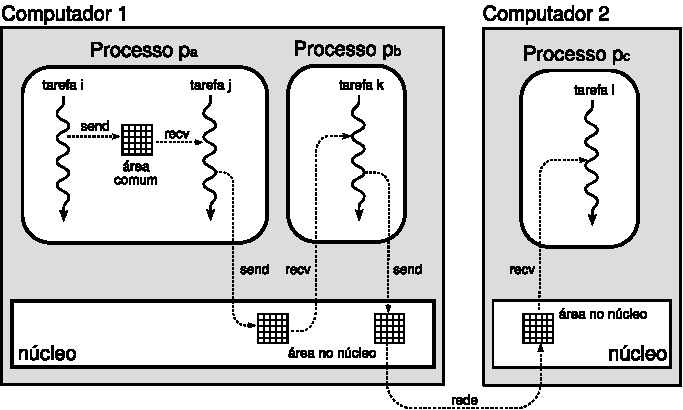
\includegraphics[width=12cm]{exemplo-figura.pdf}
\caption{Comunicação inter-processos.}
\label{fig:comun-intra-inter}
\end{figure}

Para mais informações consulte \cite{goossens93}.

%=====================================================

\section{Exemplo de tabela}

Tabelas são elementos importantes de um documento. No \LaTeX\ as tabelas podem ser objetos flutuantes (definidas no ambiente \texttt{table} e referenciadas por números usando \texttt{label} e \texttt{ref}) ou objetos fixos simples, criados pelo ambiente \texttt{tabular}. A tabela \ref{tab:modelos} é um exemplo de tabela flutuante, cuja posição no texto pode variar em função das quebras de página.

\begin{table}[!htp]
\centering
\caption{Os 16 modelos centrais do UCON$_{\mathrm{ABC}}$}
\label{tab:modelos}
\begin{tabular}{|c|cccc|}
\cline{2-5}
\multicolumn{1}{c|}{}& 0 (imutável) & 1 (\emph{pre-update}) & 2 (\emph{on-update}) & 3 (\emph{pos-update}) \\
\hline
\texttt{preA} & \textbullet & \textbullet & -- & \textbullet \\
\hline
\texttt{onA} & \textbullet & \textbullet & \textbullet & \textbullet \\
\hline
\texttt{preB} & \textbullet & \textbullet & -- & \textbullet \\
\hline
\texttt{onB} & \textbullet & \textbullet & \textbullet & \textbullet \\
\hline
\texttt{preC} & \textbullet & -- & -- & -- \\
\hline
\texttt{onC} & \textbullet & -- & -- & -- \\
\hline
\end{tabular}
\end{table}

%=====================================================

\section{Exemplo de equação}

Equações destacadas devem ser numeradas como mostra a equação \ref{eq:relatividade}:

\begin{equation}
E = m \times c^2
\label{eq:relatividade}
\end{equation}

%=====================================================

\section{Exemplos de código-fonte}

Códigos-fonte podem ser produzidos de forma simples através do ambiente \texttt{verbatim}, como mostra este exemplo:

\begin{footnotesize}
\begin{verbatim}
#include <stdio.h>

int main (int argc, char *argv[])
{
   int i ;                           // uma variavel local

   for (i=0; i< 100; i++)            // um laço for
      printf ("i vale %d\n", i) ;    // uma saída na tela
}
\end{verbatim}
\end{footnotesize}

No entanto, é preferível usar pacotes especializados para a edição ou inclusão de códigos-fonte, como o pacote \texttt{listings}. Eis um exemplo de código-fonte escrito com esse pacote:

% exemplo de código-fonte definido no próprio texto

\begin{lstlisting}
#include <stdio.h>

int main (int argc, char *argv[])
{
   int i ;                           // uma variável local

   for (i=0; i< 100; i++)            // um laço for
      printf ("i vale %d\n", i) ;    // uma saída na tela
}
\end{lstlisting}

Esse pacote também permite incluir códigos-fonte de arquivos externos. Eis um exemplo:

% exemplo de código-fonte incluso

\lstinputlisting{2-fundam/exemplo.c}

%=====================================================

\section{Exemplo de algoritmo}

Os pacotes \texttt{algorithm} e \texttt{algorithmic} permitem formatar algoritmos facilmente. Eis um exemplo:

\begin{algorithm}[H]
\caption{Ações de $s_i$ ao encerrar um ciclo:}
\label{alg:on-period-ending}
\begin{small}
\begin{algorithmic}[1]
\FORALL{$x \in \mathcal{K}_i$}
  \STATE{$\mathit{banned}_i(x) \gets$ FALSE}
  \STATE{$mi_i(x) \gets 0$}
  \STATE{$mm_i(x) \gets 0$}
  \STATE{$\mathit{age}_i(x) \gets \mathit{age}_i(x) + 1$}
  \IF{$\mathit{age}_i(x) = \mathit{age}_\mathit{max}$}
     \STATE{$\mathcal{K}_i \gets \mathcal{K}_i - \{x\}$}
     \COMMENT{``esquece'' do servidor $x$}
     \STATE{remove as informações locais sobre $x$}
     \STATE{envia $\mathit{notify}(x,\mathit{undef})$ ao grupo de confiança $\mathcal{T}_i$}
  \ENDIF
\ENDFOR
\end{algorithmic}
\end{small}
\end{algorithm}
 
%=====================================================

\section{Exemplo de citação}

Como afirmou Maquiavel em seu livro \emph{O Príncipe}:

\begin{quote}
``Nada é mais difícil de instituir, mais perigoso de conduzir, mais incerto no seu sucesso, do que liderar a introdução de uma nova ordem de coisas... O inovador faz inimigos em todos aqueles que prosperavam sobre as antigas regras, e somente tíbio suporte é esperado daqueles que prosperariam na novidade, porque os homens são geralmente incrédulos, nunca realmente confiam nas coisas novas, a menos que as tenham testado em experiência''.
\end{quote}

%=====================================================

\section{Conclusão}

Todo capítulo (com exceção da introdução e da conclusão) deve encerrar com uma pequena conclusão local, resumindo os tópicos apresentados no capítulo e preparando o leitor para o próximo capítulo (exceto se esse for a conclusão geral). Caso o capítulo tenha apresentado resultados obtidos pelo próprio autor, estes devem ser sucintamente relembrados aqui.

%=====================================================
			% estado da arte
%\chapter{Alguns exemplos}
\label{cap:exemplos}

% figuras estão no subdiretório "figuras/" dentro deste capítulo
\graphicspath{\currfiledir/figuras/}

%=====================================================

\section{Guias de \LaTeX}

Este modelo contém exemplos para os padrões de inserção de figuras, tabelas, listas de itens, bibliografia, etc. Em caso de dúvidas ou discordância, Pode-se entrar em contato com a direção ou secretaria do programa. Obviamente, críticas (construtivas) e sugestões são muito bem-vindas.

Para aprender a usar \LaTeX, um bom guia introdutório disponível na Internet é \cite{oetiker07}, que também tem uma versão em português. Para tópicos mais avançados consulte \cite{goossens93}.

%=====================================================

\section{Estrutura do texto}

Para melhorar a legibilidade do texto, deve ser extremamente evitado o uso de subdivisões mais profundas que a subseção (por exemplo, subsubseções). Se elas forem absolutamente necessarias, não devem ser numeradas. Deve-se analisar a possibilidade de uso de uma lista de itens em seu lugar. O número de níveis de texto do documento não deve exceder três: capítulo, seção e subseção. O uso de mais que três níveis dificulta a leitura e prejudica muito a estética do texto.

%=====================================================

\section{Estilo de redação}

Ao elaborar o texto da dissertação ou da tese, o mais indicado é o uso do verbo na forma impessoal. Exemplos:

\begin{itemize}
\item ... utilizaram-se os seguintes dados ...
\item ... elaborou-se de forma precisa ...
\item ... trata-se os algoritmos ...
\item ... foram obtidos resultados significativos ...
\end{itemize}

Além disso, deve-se a todo custo evitar a ``linguagem de revista'', com expressões como ``sensacional'', ``impressionante'', ``monstruoso'', etc (por exemplo: ``Os resultados obtidos são sensacionais, sobretudo considerando a monstruosa margem de erro.'').

%=====================================================

\section{Exemplo de figura}

A forma sugerida para incluir figuras em um documento \LaTeX\ é importá-las usando o pacote \texttt{graphicx}. Como formatos gráficos sugere-se:

\begin{itemize}

\item Formatos \emph{raster}, como PNG (\emph{Portable Network Graphics}) ou JPG (\emph{Joint Photographic Experts Group}) para fotografias; procure usar uma resolução de ao menos 150 dpi (\emph{dots per inch}).

\item Formatos vetoriais, como PDF (\emph{Portable Document Format}) ou EPS (\emph{Extended PostScript}) para diagramas e gráficos\footnote{NUNCA use JPG ou GIF para desenhos vetoriais, pois o resultado final geralmente fica borrado.}.

\end{itemize}

A maior parte das ferramentas permite exportar figuras nesses formatos (a figura do exemplo foi produzida com o \emph{Inkscape}, um programa livre multiplataforma). A figura \ref{fig:comun-intra-inter} mostra um exemplo de inclusão de figura em PDF.

% exemplo de inserção de figura
\begin{figure}[!htb]
\centering
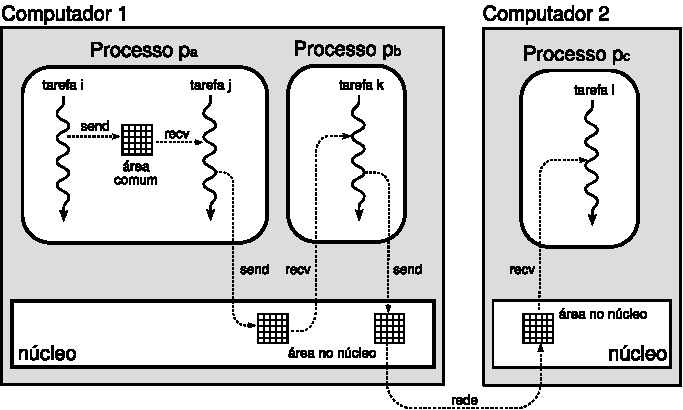
\includegraphics[width=12cm]{exemplo-figura.pdf}
\caption{Comunicação inter-processos.}
\label{fig:comun-intra-inter}
\end{figure}

Para mais informações consulte \cite{goossens93}.

%=====================================================

\section{Exemplo de tabela}

Tabelas são elementos importantes de um documento. No \LaTeX\ as tabelas podem ser objetos flutuantes (definidas no ambiente \texttt{table} e referenciadas por números usando \texttt{label} e \texttt{ref}) ou objetos fixos simples, criados pelo ambiente \texttt{tabular}. A tabela \ref{tab:modelos} é um exemplo de tabela flutuante, cuja posição no texto pode variar em função das quebras de página.

\begin{table}[!htp]
\centering
\caption{Os 16 modelos centrais do UCON$_{\mathrm{ABC}}$}
\label{tab:modelos}
\begin{tabular}{|c|cccc|}
\cline{2-5}
\multicolumn{1}{c|}{}& 0 (imutável) & 1 (\emph{pre-update}) & 2 (\emph{on-update}) & 3 (\emph{pos-update}) \\
\hline
\texttt{preA} & \textbullet & \textbullet & -- & \textbullet \\
\hline
\texttt{onA} & \textbullet & \textbullet & \textbullet & \textbullet \\
\hline
\texttt{preB} & \textbullet & \textbullet & -- & \textbullet \\
\hline
\texttt{onB} & \textbullet & \textbullet & \textbullet & \textbullet \\
\hline
\texttt{preC} & \textbullet & -- & -- & -- \\
\hline
\texttt{onC} & \textbullet & -- & -- & -- \\
\hline
\end{tabular}
\end{table}

%=====================================================

\section{Exemplo de equação}

Equações destacadas devem ser numeradas como mostra a equação \ref{eq:relatividade}:

\begin{equation}
E = m \times c^2
\label{eq:relatividade}
\end{equation}

%=====================================================

\section{Exemplos de código-fonte}

Códigos-fonte podem ser produzidos de forma simples através do ambiente \texttt{verbatim}, como mostra este exemplo:

\begin{footnotesize}
\begin{verbatim}
#include <stdio.h>

int main (int argc, char *argv[])
{
   int i ;                           // uma variavel local

   for (i=0; i< 100; i++)            // um laço for
      printf ("i vale %d\n", i) ;    // uma saída na tela
}
\end{verbatim}
\end{footnotesize}

No entanto, é preferível usar pacotes especializados para a edição ou inclusão de códigos-fonte, como o pacote \texttt{listings}. Eis um exemplo de código-fonte escrito com esse pacote:

% exemplo de código-fonte definido no próprio texto

\begin{lstlisting}
#include <stdio.h>

int main (int argc, char *argv[])
{
   int i ;                           // uma variável local

   for (i=0; i< 100; i++)            // um laço for
      printf ("i vale %d\n", i) ;    // uma saída na tela
}
\end{lstlisting}

Esse pacote também permite incluir códigos-fonte de arquivos externos. Eis um exemplo:

% exemplo de código-fonte incluso

\lstinputlisting{2-fundam/exemplo.c}

%=====================================================

\section{Exemplo de algoritmo}

Os pacotes \texttt{algorithm} e \texttt{algorithmic} permitem formatar algoritmos facilmente. Eis um exemplo:

\begin{algorithm}[H]
\caption{Ações de $s_i$ ao encerrar um ciclo:}
\label{alg:on-period-ending}
\begin{small}
\begin{algorithmic}[1]
\FORALL{$x \in \mathcal{K}_i$}
  \STATE{$\mathit{banned}_i(x) \gets$ FALSE}
  \STATE{$mi_i(x) \gets 0$}
  \STATE{$mm_i(x) \gets 0$}
  \STATE{$\mathit{age}_i(x) \gets \mathit{age}_i(x) + 1$}
  \IF{$\mathit{age}_i(x) = \mathit{age}_\mathit{max}$}
     \STATE{$\mathcal{K}_i \gets \mathcal{K}_i - \{x\}$}
     \COMMENT{``esquece'' do servidor $x$}
     \STATE{remove as informações locais sobre $x$}
     \STATE{envia $\mathit{notify}(x,\mathit{undef})$ ao grupo de confiança $\mathcal{T}_i$}
  \ENDIF
\ENDFOR
\end{algorithmic}
\end{small}
\end{algorithm}
 
%=====================================================

\section{Exemplo de citação}

Como afirmou Maquiavel em seu livro \emph{O Príncipe}:

\begin{quote}
``Nada é mais difícil de instituir, mais perigoso de conduzir, mais incerto no seu sucesso, do que liderar a introdução de uma nova ordem de coisas... O inovador faz inimigos em todos aqueles que prosperavam sobre as antigas regras, e somente tíbio suporte é esperado daqueles que prosperariam na novidade, porque os homens são geralmente incrédulos, nunca realmente confiam nas coisas novas, a menos que as tenham testado em experiência''.
\end{quote}

%=====================================================

\section{Conclusão}

Todo capítulo (com exceção da introdução e da conclusão) deve encerrar com uma pequena conclusão local, resumindo os tópicos apresentados no capítulo e preparando o leitor para o próximo capítulo (exceto se esse for a conclusão geral). Caso o capítulo tenha apresentado resultados obtidos pelo próprio autor, estes devem ser sucintamente relembrados aqui.

%=====================================================
		% proposta
%\chapter{Alguns exemplos}
\label{cap:exemplos}

% figuras estão no subdiretório "figuras/" dentro deste capítulo
\graphicspath{\currfiledir/figuras/}

%=====================================================

\section{Guias de \LaTeX}

Este modelo contém exemplos para os padrões de inserção de figuras, tabelas, listas de itens, bibliografia, etc. Em caso de dúvidas ou discordância, Pode-se entrar em contato com a direção ou secretaria do programa. Obviamente, críticas (construtivas) e sugestões são muito bem-vindas.

Para aprender a usar \LaTeX, um bom guia introdutório disponível na Internet é \cite{oetiker07}, que também tem uma versão em português. Para tópicos mais avançados consulte \cite{goossens93}.

%=====================================================

\section{Estrutura do texto}

Para melhorar a legibilidade do texto, deve ser extremamente evitado o uso de subdivisões mais profundas que a subseção (por exemplo, subsubseções). Se elas forem absolutamente necessarias, não devem ser numeradas. Deve-se analisar a possibilidade de uso de uma lista de itens em seu lugar. O número de níveis de texto do documento não deve exceder três: capítulo, seção e subseção. O uso de mais que três níveis dificulta a leitura e prejudica muito a estética do texto.

%=====================================================

\section{Estilo de redação}

Ao elaborar o texto da dissertação ou da tese, o mais indicado é o uso do verbo na forma impessoal. Exemplos:

\begin{itemize}
\item ... utilizaram-se os seguintes dados ...
\item ... elaborou-se de forma precisa ...
\item ... trata-se os algoritmos ...
\item ... foram obtidos resultados significativos ...
\end{itemize}

Além disso, deve-se a todo custo evitar a ``linguagem de revista'', com expressões como ``sensacional'', ``impressionante'', ``monstruoso'', etc (por exemplo: ``Os resultados obtidos são sensacionais, sobretudo considerando a monstruosa margem de erro.'').

%=====================================================

\section{Exemplo de figura}

A forma sugerida para incluir figuras em um documento \LaTeX\ é importá-las usando o pacote \texttt{graphicx}. Como formatos gráficos sugere-se:

\begin{itemize}

\item Formatos \emph{raster}, como PNG (\emph{Portable Network Graphics}) ou JPG (\emph{Joint Photographic Experts Group}) para fotografias; procure usar uma resolução de ao menos 150 dpi (\emph{dots per inch}).

\item Formatos vetoriais, como PDF (\emph{Portable Document Format}) ou EPS (\emph{Extended PostScript}) para diagramas e gráficos\footnote{NUNCA use JPG ou GIF para desenhos vetoriais, pois o resultado final geralmente fica borrado.}.

\end{itemize}

A maior parte das ferramentas permite exportar figuras nesses formatos (a figura do exemplo foi produzida com o \emph{Inkscape}, um programa livre multiplataforma). A figura \ref{fig:comun-intra-inter} mostra um exemplo de inclusão de figura em PDF.

% exemplo de inserção de figura
\begin{figure}[!htb]
\centering
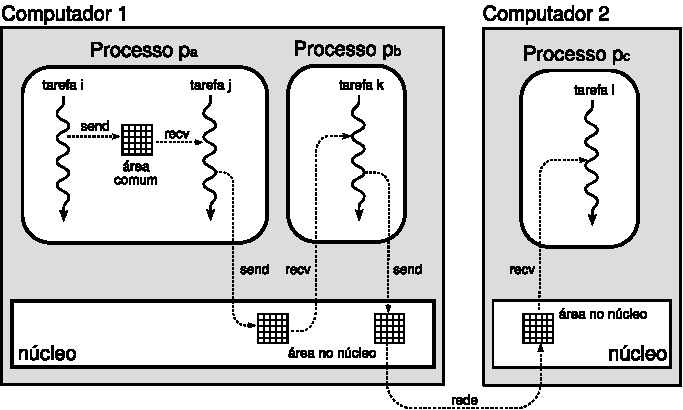
\includegraphics[width=12cm]{exemplo-figura.pdf}
\caption{Comunicação inter-processos.}
\label{fig:comun-intra-inter}
\end{figure}

Para mais informações consulte \cite{goossens93}.

%=====================================================

\section{Exemplo de tabela}

Tabelas são elementos importantes de um documento. No \LaTeX\ as tabelas podem ser objetos flutuantes (definidas no ambiente \texttt{table} e referenciadas por números usando \texttt{label} e \texttt{ref}) ou objetos fixos simples, criados pelo ambiente \texttt{tabular}. A tabela \ref{tab:modelos} é um exemplo de tabela flutuante, cuja posição no texto pode variar em função das quebras de página.

\begin{table}[!htp]
\centering
\caption{Os 16 modelos centrais do UCON$_{\mathrm{ABC}}$}
\label{tab:modelos}
\begin{tabular}{|c|cccc|}
\cline{2-5}
\multicolumn{1}{c|}{}& 0 (imutável) & 1 (\emph{pre-update}) & 2 (\emph{on-update}) & 3 (\emph{pos-update}) \\
\hline
\texttt{preA} & \textbullet & \textbullet & -- & \textbullet \\
\hline
\texttt{onA} & \textbullet & \textbullet & \textbullet & \textbullet \\
\hline
\texttt{preB} & \textbullet & \textbullet & -- & \textbullet \\
\hline
\texttt{onB} & \textbullet & \textbullet & \textbullet & \textbullet \\
\hline
\texttt{preC} & \textbullet & -- & -- & -- \\
\hline
\texttt{onC} & \textbullet & -- & -- & -- \\
\hline
\end{tabular}
\end{table}

%=====================================================

\section{Exemplo de equação}

Equações destacadas devem ser numeradas como mostra a equação \ref{eq:relatividade}:

\begin{equation}
E = m \times c^2
\label{eq:relatividade}
\end{equation}

%=====================================================

\section{Exemplos de código-fonte}

Códigos-fonte podem ser produzidos de forma simples através do ambiente \texttt{verbatim}, como mostra este exemplo:

\begin{footnotesize}
\begin{verbatim}
#include <stdio.h>

int main (int argc, char *argv[])
{
   int i ;                           // uma variavel local

   for (i=0; i< 100; i++)            // um laço for
      printf ("i vale %d\n", i) ;    // uma saída na tela
}
\end{verbatim}
\end{footnotesize}

No entanto, é preferível usar pacotes especializados para a edição ou inclusão de códigos-fonte, como o pacote \texttt{listings}. Eis um exemplo de código-fonte escrito com esse pacote:

% exemplo de código-fonte definido no próprio texto

\begin{lstlisting}
#include <stdio.h>

int main (int argc, char *argv[])
{
   int i ;                           // uma variável local

   for (i=0; i< 100; i++)            // um laço for
      printf ("i vale %d\n", i) ;    // uma saída na tela
}
\end{lstlisting}

Esse pacote também permite incluir códigos-fonte de arquivos externos. Eis um exemplo:

% exemplo de código-fonte incluso

\lstinputlisting{2-fundam/exemplo.c}

%=====================================================

\section{Exemplo de algoritmo}

Os pacotes \texttt{algorithm} e \texttt{algorithmic} permitem formatar algoritmos facilmente. Eis um exemplo:

\begin{algorithm}[H]
\caption{Ações de $s_i$ ao encerrar um ciclo:}
\label{alg:on-period-ending}
\begin{small}
\begin{algorithmic}[1]
\FORALL{$x \in \mathcal{K}_i$}
  \STATE{$\mathit{banned}_i(x) \gets$ FALSE}
  \STATE{$mi_i(x) \gets 0$}
  \STATE{$mm_i(x) \gets 0$}
  \STATE{$\mathit{age}_i(x) \gets \mathit{age}_i(x) + 1$}
  \IF{$\mathit{age}_i(x) = \mathit{age}_\mathit{max}$}
     \STATE{$\mathcal{K}_i \gets \mathcal{K}_i - \{x\}$}
     \COMMENT{``esquece'' do servidor $x$}
     \STATE{remove as informações locais sobre $x$}
     \STATE{envia $\mathit{notify}(x,\mathit{undef})$ ao grupo de confiança $\mathcal{T}_i$}
  \ENDIF
\ENDFOR
\end{algorithmic}
\end{small}
\end{algorithm}
 
%=====================================================

\section{Exemplo de citação}

Como afirmou Maquiavel em seu livro \emph{O Príncipe}:

\begin{quote}
``Nada é mais difícil de instituir, mais perigoso de conduzir, mais incerto no seu sucesso, do que liderar a introdução de uma nova ordem de coisas... O inovador faz inimigos em todos aqueles que prosperavam sobre as antigas regras, e somente tíbio suporte é esperado daqueles que prosperariam na novidade, porque os homens são geralmente incrédulos, nunca realmente confiam nas coisas novas, a menos que as tenham testado em experiência''.
\end{quote}

%=====================================================

\section{Conclusão}

Todo capítulo (com exceção da introdução e da conclusão) deve encerrar com uma pequena conclusão local, resumindo os tópicos apresentados no capítulo e preparando o leitor para o próximo capítulo (exceto se esse for a conclusão geral). Caso o capítulo tenha apresentado resultados obtidos pelo próprio autor, estes devem ser sucintamente relembrados aqui.

%=====================================================
		% experimentação e validação
%\chapter{Alguns exemplos}
\label{cap:exemplos}

% figuras estão no subdiretório "figuras/" dentro deste capítulo
\graphicspath{\currfiledir/figuras/}

%=====================================================

\section{Guias de \LaTeX}

Este modelo contém exemplos para os padrões de inserção de figuras, tabelas, listas de itens, bibliografia, etc. Em caso de dúvidas ou discordância, Pode-se entrar em contato com a direção ou secretaria do programa. Obviamente, críticas (construtivas) e sugestões são muito bem-vindas.

Para aprender a usar \LaTeX, um bom guia introdutório disponível na Internet é \cite{oetiker07}, que também tem uma versão em português. Para tópicos mais avançados consulte \cite{goossens93}.

%=====================================================

\section{Estrutura do texto}

Para melhorar a legibilidade do texto, deve ser extremamente evitado o uso de subdivisões mais profundas que a subseção (por exemplo, subsubseções). Se elas forem absolutamente necessarias, não devem ser numeradas. Deve-se analisar a possibilidade de uso de uma lista de itens em seu lugar. O número de níveis de texto do documento não deve exceder três: capítulo, seção e subseção. O uso de mais que três níveis dificulta a leitura e prejudica muito a estética do texto.

%=====================================================

\section{Estilo de redação}

Ao elaborar o texto da dissertação ou da tese, o mais indicado é o uso do verbo na forma impessoal. Exemplos:

\begin{itemize}
\item ... utilizaram-se os seguintes dados ...
\item ... elaborou-se de forma precisa ...
\item ... trata-se os algoritmos ...
\item ... foram obtidos resultados significativos ...
\end{itemize}

Além disso, deve-se a todo custo evitar a ``linguagem de revista'', com expressões como ``sensacional'', ``impressionante'', ``monstruoso'', etc (por exemplo: ``Os resultados obtidos são sensacionais, sobretudo considerando a monstruosa margem de erro.'').

%=====================================================

\section{Exemplo de figura}

A forma sugerida para incluir figuras em um documento \LaTeX\ é importá-las usando o pacote \texttt{graphicx}. Como formatos gráficos sugere-se:

\begin{itemize}

\item Formatos \emph{raster}, como PNG (\emph{Portable Network Graphics}) ou JPG (\emph{Joint Photographic Experts Group}) para fotografias; procure usar uma resolução de ao menos 150 dpi (\emph{dots per inch}).

\item Formatos vetoriais, como PDF (\emph{Portable Document Format}) ou EPS (\emph{Extended PostScript}) para diagramas e gráficos\footnote{NUNCA use JPG ou GIF para desenhos vetoriais, pois o resultado final geralmente fica borrado.}.

\end{itemize}

A maior parte das ferramentas permite exportar figuras nesses formatos (a figura do exemplo foi produzida com o \emph{Inkscape}, um programa livre multiplataforma). A figura \ref{fig:comun-intra-inter} mostra um exemplo de inclusão de figura em PDF.

% exemplo de inserção de figura
\begin{figure}[!htb]
\centering
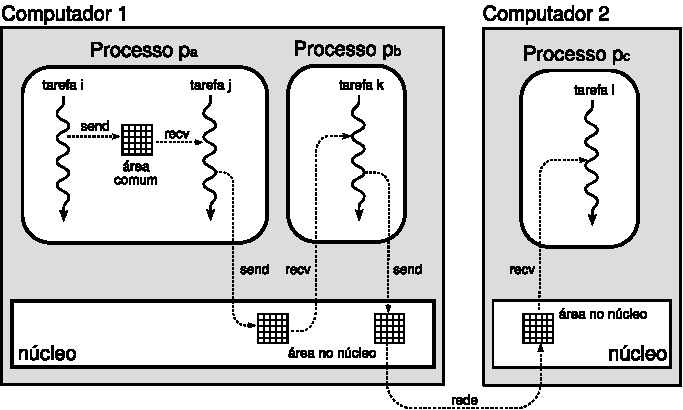
\includegraphics[width=12cm]{exemplo-figura.pdf}
\caption{Comunicação inter-processos.}
\label{fig:comun-intra-inter}
\end{figure}

Para mais informações consulte \cite{goossens93}.

%=====================================================

\section{Exemplo de tabela}

Tabelas são elementos importantes de um documento. No \LaTeX\ as tabelas podem ser objetos flutuantes (definidas no ambiente \texttt{table} e referenciadas por números usando \texttt{label} e \texttt{ref}) ou objetos fixos simples, criados pelo ambiente \texttt{tabular}. A tabela \ref{tab:modelos} é um exemplo de tabela flutuante, cuja posição no texto pode variar em função das quebras de página.

\begin{table}[!htp]
\centering
\caption{Os 16 modelos centrais do UCON$_{\mathrm{ABC}}$}
\label{tab:modelos}
\begin{tabular}{|c|cccc|}
\cline{2-5}
\multicolumn{1}{c|}{}& 0 (imutável) & 1 (\emph{pre-update}) & 2 (\emph{on-update}) & 3 (\emph{pos-update}) \\
\hline
\texttt{preA} & \textbullet & \textbullet & -- & \textbullet \\
\hline
\texttt{onA} & \textbullet & \textbullet & \textbullet & \textbullet \\
\hline
\texttt{preB} & \textbullet & \textbullet & -- & \textbullet \\
\hline
\texttt{onB} & \textbullet & \textbullet & \textbullet & \textbullet \\
\hline
\texttt{preC} & \textbullet & -- & -- & -- \\
\hline
\texttt{onC} & \textbullet & -- & -- & -- \\
\hline
\end{tabular}
\end{table}

%=====================================================

\section{Exemplo de equação}

Equações destacadas devem ser numeradas como mostra a equação \ref{eq:relatividade}:

\begin{equation}
E = m \times c^2
\label{eq:relatividade}
\end{equation}

%=====================================================

\section{Exemplos de código-fonte}

Códigos-fonte podem ser produzidos de forma simples através do ambiente \texttt{verbatim}, como mostra este exemplo:

\begin{footnotesize}
\begin{verbatim}
#include <stdio.h>

int main (int argc, char *argv[])
{
   int i ;                           // uma variavel local

   for (i=0; i< 100; i++)            // um laço for
      printf ("i vale %d\n", i) ;    // uma saída na tela
}
\end{verbatim}
\end{footnotesize}

No entanto, é preferível usar pacotes especializados para a edição ou inclusão de códigos-fonte, como o pacote \texttt{listings}. Eis um exemplo de código-fonte escrito com esse pacote:

% exemplo de código-fonte definido no próprio texto

\begin{lstlisting}
#include <stdio.h>

int main (int argc, char *argv[])
{
   int i ;                           // uma variável local

   for (i=0; i< 100; i++)            // um laço for
      printf ("i vale %d\n", i) ;    // uma saída na tela
}
\end{lstlisting}

Esse pacote também permite incluir códigos-fonte de arquivos externos. Eis um exemplo:

% exemplo de código-fonte incluso

\lstinputlisting{2-fundam/exemplo.c}

%=====================================================

\section{Exemplo de algoritmo}

Os pacotes \texttt{algorithm} e \texttt{algorithmic} permitem formatar algoritmos facilmente. Eis um exemplo:

\begin{algorithm}[H]
\caption{Ações de $s_i$ ao encerrar um ciclo:}
\label{alg:on-period-ending}
\begin{small}
\begin{algorithmic}[1]
\FORALL{$x \in \mathcal{K}_i$}
  \STATE{$\mathit{banned}_i(x) \gets$ FALSE}
  \STATE{$mi_i(x) \gets 0$}
  \STATE{$mm_i(x) \gets 0$}
  \STATE{$\mathit{age}_i(x) \gets \mathit{age}_i(x) + 1$}
  \IF{$\mathit{age}_i(x) = \mathit{age}_\mathit{max}$}
     \STATE{$\mathcal{K}_i \gets \mathcal{K}_i - \{x\}$}
     \COMMENT{``esquece'' do servidor $x$}
     \STATE{remove as informações locais sobre $x$}
     \STATE{envia $\mathit{notify}(x,\mathit{undef})$ ao grupo de confiança $\mathcal{T}_i$}
  \ENDIF
\ENDFOR
\end{algorithmic}
\end{small}
\end{algorithm}
 
%=====================================================

\section{Exemplo de citação}

Como afirmou Maquiavel em seu livro \emph{O Príncipe}:

\begin{quote}
``Nada é mais difícil de instituir, mais perigoso de conduzir, mais incerto no seu sucesso, do que liderar a introdução de uma nova ordem de coisas... O inovador faz inimigos em todos aqueles que prosperavam sobre as antigas regras, e somente tíbio suporte é esperado daqueles que prosperariam na novidade, porque os homens são geralmente incrédulos, nunca realmente confiam nas coisas novas, a menos que as tenham testado em experiência''.
\end{quote}

%=====================================================

\section{Conclusão}

Todo capítulo (com exceção da introdução e da conclusão) deve encerrar com uma pequena conclusão local, resumindo os tópicos apresentados no capítulo e preparando o leitor para o próximo capítulo (exceto se esse for a conclusão geral). Caso o capítulo tenha apresentado resultados obtidos pelo próprio autor, estes devem ser sucintamente relembrados aqui.

%=====================================================
		% conclusão

%=====================================================

% Estilos de bibliografia recomendados (só descomentar um estilo!)
% Mais infos: https://pt.sharelatex.com/learn/Bibtex_bibliography_styles
%
% ATENÇÃO: evite usar \cite{}; prefira \citep{} e \citet{}
%
\bibliographystyle{apalike-ptbr}	% [Maziero et al., 2006]
%\bibliographystyle{alpha}		% [Maz06]
%\bibliographystyle{plainnat}		% vide Google "LaTeX Natbib"
%\bibliographystyle{plain}		% [1] ordem alfabética
%\bibliographystyle{unsrt}		% [1] ordem de uso no texto

% no estilo "unsrt", evita que citações nos índices sejam consideradas
%\usepackage{notoccite}

% base de bibliografia (BibTeX)
\bibliography{referencias}
%\bibliography{file1,file2,file3} % se tiver mais de um arquivo BibTeX

%=====================================================

% inclusão de apêndices
\appendix

% inclusão de apêndice
\chapter{Exemplo de anexo}

%=====================================================

Os apêndices são uma extensão do texto, destacados deste para evitar descontinuidade na sequência lógica ou alongamento excessivo de determinado assunto ou tópico secundário dentro dos capítulos da dissertação ou da tese. São contribuições que servem para esclarecer, complementar, provar ou confirmar as ideias apresentadas no texto dos capítulos e que são importantes para a compreensão dos mesmos.

Todos os apêndices devem vir após as referências bibliográficas e devem ser enumerados por letras maiúsculas (A, B, C, ...).

%=====================================================

\section{Uma Seção}

\lipsum[20-23]

%=====================================================

\subsection{Uma sub-Seção}

\lipsum[30-33]

%=====================================================

\subsection{Outra sub-Seção}

Exemplo de lista simples com dois níveis: Exemplo de lista simples com dois níveis: Exemplo de lista simples com dois níveis: Exemplo de lista simples com dois níveis: Exemplo de lista simples com dois níveis: Exemplo de lista simples com dois níveis: Exemplo de lista simples com dois níveis: Exemplo de lista simples com dois níveis: Exemplo de lista simples com dois níveis.

\begin{itemize}

\item Banana, Banana, Banana, Banana, Banana, Banana, Banana, Banana, Banana, Banana, Banana, Banana, Banana, Banana, Banana, Banana, Banana, Banana, Banana, Banana, Banana, Banana, Banana, Banana.

\begin{itemize}

\item Caturra, Caturra, Caturra, Caturra, Caturra, Caturra, Caturra, Caturra, Caturra, Caturra, Caturra, Caturra, Caturra, Caturra, Caturra, Caturra, Caturra, Caturra, Caturra.

\item da Terra, da Terra, da Terra, da Terra, da Terra, da Terra, da Terra, da Terra, da Terra, da Terra, da Terra, da Terra, da Terra, da Terra, da Terra, da Terra, da Terra, da Terra.

\end{itemize}

\item Laranja, Laranja, Laranja, Laranja, Laranja, Laranja, Laranja, Laranja, Laranja, Laranja, Laranja, Laranja, Laranja, Laranja, Laranja, Laranja.

\begin{itemize}

\item Bahia, Bahia, Bahia, Bahia, Bahia, Bahia, Bahia, Bahia, Bahia, Bahia, Bahia, Bahia, Bahia, Bahia, Bahia, Bahia, Bahia, Bahia.

\item Lima, Lima, Lima, Lima, Lima, Lima, Lima, Lima, Lima, Lima, Lima, Lima, Lima, Lima, Lima, Lima, Lima, Lima, Lima, Lima, Lima, Lima, Lima, Lima, Lima, Lima, Lima, Lima, Lima.

\end{itemize}

\end{itemize}

Exemplo de lista numerada com dois níveis: Exemplo de lista numerada com dois níveis: Exemplo de lista numerada com dois níveis: Exemplo de lista numerada com dois níveis: Exemplo de lista numerada com dois níveis: Exemplo de lista numerada com dois níveis: Exemplo de lista numerada com dois níveis: Exemplo de lista numerada com dois níveis.

\begin{enumerate}

\item Banana, Banana, Banana, Banana, Banana, Banana, Banana, Banana, Banana, Banana, Banana, Banana, Banana, Banana, Banana, Banana, Banana, Banana, Banana, Banana, Banana, Banana, Banana, Banana.

\begin{enumerate}

\item Caturra, Caturra, Caturra, Caturra, Caturra, Caturra, Caturra, Caturra, Caturra, Caturra, Caturra, Caturra, Caturra, Caturra, Caturra, Caturra, Caturra, Caturra, Caturra.

\item da Terra, da Terra, da Terra, da Terra, da Terra, da Terra, da Terra, da Terra, da Terra, da Terra, da Terra, da Terra, da Terra, da Terra, da Terra, da Terra, da Terra, da Terra.

\end{enumerate}

\item Laranja, Laranja, Laranja, Laranja, Laranja, Laranja, Laranja, Laranja, Laranja, Laranja, Laranja, Laranja, Laranja, Laranja, Laranja, Laranja.

\begin{enumerate}

\item Bahia, Bahia, Bahia, Bahia, Bahia, Bahia, Bahia, Bahia, Bahia, Bahia, Bahia, Bahia, Bahia, Bahia, Bahia, Bahia, Bahia, Bahia.

\item Lima, Lima, Lima, Lima, Lima, Lima, Lima, Lima, Lima, Lima, Lima, Lima, Lima, Lima, Lima, Lima, Lima, Lima, Lima, Lima, Lima, Lima, Lima, Lima, Lima, Lima, Lima, Lima, Lima.

\end{enumerate}

\end{enumerate}

Exemplo de lista descritiva com dois níveis: Exemplo de lista descritiva com dois níveis: Exemplo de lista descritiva com dois níveis: Exemplo de lista descritiva com dois níveis: Exemplo de lista descritiva com dois níveis: Exemplo de lista descritiva com dois níveis: Exemplo de lista descritiva com dois níveis: Exemplo de lista descritiva com dois níveis: Exemplo de lista descritiva com dois níveis.

\begin{description}

\item [Banana]: Banana, Banana, Banana, Banana, Banana, Banana, Banana, Banana, Banana, Banana, Banana, Banana, Banana, Banana, Banana, Banana, Banana, Banana, Banana, Banana, Banana, Banana, Banana.

\begin{description}

\item [Caturra]: Caturra, Caturra, Caturra, Caturra, Caturra, Caturra, Caturra, Caturra, Caturra, Caturra, Caturra, Caturra, Caturra, Caturra, Caturra, Caturra, Caturra, Caturra.

\item [da Terra]: da Terra, da Terra, da Terra, da Terra, da Terra, da Terra, da Terra, da Terra, da Terra, da Terra, da Terra, da Terra, da Terra, da Terra, da Terra, da Terra, da Terra.

\end{description}

\item [Laranja]: Laranja, Laranja, Laranja, Laranja, Laranja, Laranja, Laranja, Laranja, Laranja, Laranja, Laranja, Laranja, Laranja, Laranja, Laranja.

\begin{description}

\item [Bahia]: Bahia, Bahia, Bahia, Bahia, Bahia, Bahia, Bahia, Bahia, Bahia, Bahia, Bahia, Bahia, Bahia, Bahia, Bahia, Bahia, Bahia.

\item [Lima]: Lima, Lima, Lima, Lima, Lima, Lima, Lima, Lima, Lima, Lima, Lima, Lima, Lima, Lima, Lima, Lima, Lima, Lima, Lima, Lima, Lima, Lima, Lima, Lima, Lima, Lima, Lima, Lima.

\end{description}

\end{description}

%=====================================================


% inclusão de apêndice
\chapter{Testes de alinhamento de listas}

%=====================================================

\section{Outra seção}

Exemplo de lista simples com dois níveis: Exemplo de lista simples com dois níveis: Exemplo de lista simples com dois níveis: Exemplo de lista simples com dois níveis: Exemplo de lista simples com dois níveis: Exemplo de lista simples com dois níveis: Exemplo de lista simples com dois níveis: Exemplo de lista simples com dois níveis: Exemplo de lista simples com dois níveis.

\begin{itemize}

\item Banana, Banana, Banana, Banana, Banana, Banana, Banana, Banana, Banana, Banana, Banana, Banana, Banana, Banana, Banana, Banana, Banana, Banana, Banana, Banana, Banana, Banana, Banana, Banana.

\begin{itemize}

\item Caturra, Caturra, Caturra, Caturra, Caturra, Caturra, Caturra, Caturra, Caturra, Caturra, Caturra, Caturra, Caturra, Caturra, Caturra, Caturra, Caturra, Caturra, Caturra.

\item da Terra, da Terra, da Terra, da Terra, da Terra, da Terra, da Terra, da Terra, da Terra, da Terra, da Terra, da Terra, da Terra, da Terra, da Terra, da Terra, da Terra, da Terra.

\end{itemize}

\item Laranja, Laranja, Laranja, Laranja, Laranja, Laranja, Laranja, Laranja, Laranja, Laranja, Laranja, Laranja, Laranja, Laranja, Laranja, Laranja.

\begin{itemize}

\item Bahia, Bahia, Bahia, Bahia, Bahia, Bahia, Bahia, Bahia, Bahia, Bahia, Bahia, Bahia, Bahia, Bahia, Bahia, Bahia, Bahia, Bahia.

\item Lima, Lima, Lima, Lima, Lima, Lima, Lima, Lima, Lima, Lima, Lima, Lima, Lima, Lima, Lima, Lima, Lima, Lima, Lima, Lima, Lima, Lima, Lima, Lima, Lima, Lima, Lima, Lima, Lima.

\end{itemize}

\end{itemize}

Exemplo de lista numerada com dois níveis: Exemplo de lista numerada com dois níveis: Exemplo de lista numerada com dois níveis: Exemplo de lista numerada com dois níveis: Exemplo de lista numerada com dois níveis: Exemplo de lista numerada com dois níveis: Exemplo de lista numerada com dois níveis: Exemplo de lista numerada com dois níveis.

\begin{enumerate}

\item Banana, Banana, Banana, Banana, Banana, Banana, Banana, Banana, Banana, Banana, Banana, Banana, Banana, Banana, Banana, Banana, Banana, Banana, Banana, Banana, Banana, Banana, Banana, Banana.

\begin{enumerate}

\item Caturra, Caturra, Caturra, Caturra, Caturra, Caturra, Caturra, Caturra, Caturra, Caturra, Caturra, Caturra, Caturra, Caturra, Caturra, Caturra, Caturra, Caturra, Caturra.

\item da Terra, da Terra, da Terra, da Terra, da Terra, da Terra, da Terra, da Terra, da Terra, da Terra, da Terra, da Terra, da Terra, da Terra, da Terra, da Terra, da Terra, da Terra.

\end{enumerate}

\item Laranja, Laranja, Laranja, Laranja, Laranja, Laranja, Laranja, Laranja, Laranja, Laranja, Laranja, Laranja, Laranja, Laranja, Laranja, Laranja.

\begin{enumerate}

\item Bahia, Bahia, Bahia, Bahia, Bahia, Bahia, Bahia, Bahia, Bahia, Bahia, Bahia, Bahia, Bahia, Bahia, Bahia, Bahia, Bahia, Bahia.

\item Lima, Lima, Lima, Lima, Lima, Lima, Lima, Lima, Lima, Lima, Lima, Lima, Lima, Lima, Lima, Lima, Lima, Lima, Lima, Lima, Lima, Lima, Lima, Lima, Lima, Lima, Lima, Lima, Lima.

\end{enumerate}

\end{enumerate}

Exemplo de lista descritiva com dois níveis: Exemplo de lista descritiva com dois níveis: Exemplo de lista descritiva com dois níveis: Exemplo de lista descritiva com dois níveis: Exemplo de lista descritiva com dois níveis: Exemplo de lista descritiva com dois níveis: Exemplo de lista descritiva com dois níveis: Exemplo de lista descritiva com dois níveis: Exemplo de lista descritiva com dois níveis.

\begin{description}

\item [Banana]: Banana, Banana, Banana, Banana, Banana, Banana, Banana, Banana, Banana, Banana, Banana, Banana, Banana, Banana, Banana, Banana, Banana, Banana, Banana, Banana, Banana, Banana, Banana.

\begin{description}

\item [Caturra]: Caturra, Caturra, Caturra, Caturra, Caturra, Caturra, Caturra, Caturra, Caturra, Caturra, Caturra, Caturra, Caturra, Caturra, Caturra, Caturra, Caturra, Caturra.

\item [da Terra]: da Terra, da Terra, da Terra, da Terra, da Terra, da Terra, da Terra, da Terra, da Terra, da Terra, da Terra, da Terra, da Terra, da Terra, da Terra, da Terra, da Terra.

\end{description}

\item [Laranja]: Laranja, Laranja, Laranja, Laranja, Laranja, Laranja, Laranja, Laranja, Laranja, Laranja, Laranja, Laranja, Laranja, Laranja, Laranja.

\begin{description}

\item [Bahia]: Bahia, Bahia, Bahia, Bahia, Bahia, Bahia, Bahia, Bahia, Bahia, Bahia, Bahia, Bahia, Bahia, Bahia, Bahia, Bahia, Bahia.

\item [Lima]: Lima, Lima, Lima, Lima, Lima, Lima, Lima, Lima, Lima, Lima, Lima, Lima, Lima, Lima, Lima, Lima, Lima, Lima, Lima, Lima, Lima, Lima, Lima, Lima, Lima, Lima, Lima, Lima.

\end{description}

\end{description}

%=====================================================


%=====================================================

\end{document}

%=====================================================
